\documentclass[12pt,fleqn]{article}\usepackage{../../common}
\begin{document}
Dairesel Baz Fonksiyonlari (Radial Basis Functions)

\begin{minted}[fontsize=\footnotesize]{python}
from mpl_toolkits.mplot3d import Axes3D
import matplotlib.pyplot as plt
from matplotlib import cm
import numpy as np
import matplotlib.pyplot as plt
import numpy.linalg as lin
from scipy.spatial.distance import cdist
\end{minted}

\begin{minted}[fontsize=\footnotesize]{python}
np.random.seed(0)

def func(x, y):
    s1 = 0.2; x1 = 36.5; y1 = 32.5
    g1 = np.exp( -4 *np.log(2) * ((x-x1)**2+(y-y1)**2) / s1**2)
    s2 = 0.4; x2 = 36.1; y2 = 32.8
    g1 = np.exp( -4 *np.log(2) * ((x-x1)**2+(y-y1)**2) / s1**2)
    g2 = np.exp( -2 *np.log(2) * ((x-x2)**2+(y-y2)**2) / s2**2)    
    return g1 + g2 

D = 50
S = 100
gamma = 2.0

x = np.linspace(36,37,D)
y = np.linspace(32,33,D)

xx,yy = np.meshgrid(x,y)
zz = func(xx,yy)

fig = plt.figure()
ax = fig.gca(projection='3d')
surf = ax.plot_surface(xx, yy, zz, cmap=cm.coolwarm,linewidth=0, antialiased=False)
fig.colorbar(surf, shrink=0.5, aspect=5)
plt.savefig('linear_app88rbf_01.png')
\end{minted}

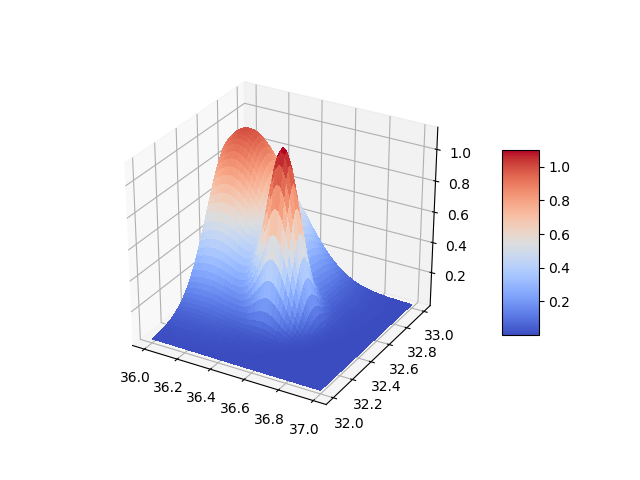
\includegraphics[width=20em]{linear_app88rbf_01.png}

\begin{minted}[fontsize=\footnotesize]{python}
xxx = xx.reshape(D*D)
yyy = yy.reshape(D*D)
zzz = zz.reshape(D*D)

idx = np.random.choice(range(D*D),S)

xr = xxx[idx].reshape(S,1)
yr = yyy[idx].reshape(S,1)
zr = zzz[idx].reshape(S,1)
X = np.hstack((xr,yr))

Phi = np.exp(-gamma*cdist(X,X,metric='euclid'))

w = np.dot(lin.pinv(Phi),zr)
a = np.vstack((xxx,yyy))
d = cdist(X,a.T)
d = np.exp(-gamma * d)
dd = np.dot(w.T,d)
znew = dd.reshape(D,D)
\end{minted}

\begin{minted}[fontsize=\footnotesize]{python}
fig = plt.figure()
ax = fig.gca(projection='3d')
surf = ax.plot_surface(xx, yy, znew, cmap=cm.coolwarm,linewidth=0, antialiased=False)
fig.colorbar(surf, shrink=0.5, aspect=5)
plt.savefig('linear_app88rbf_02.png')
\end{minted}

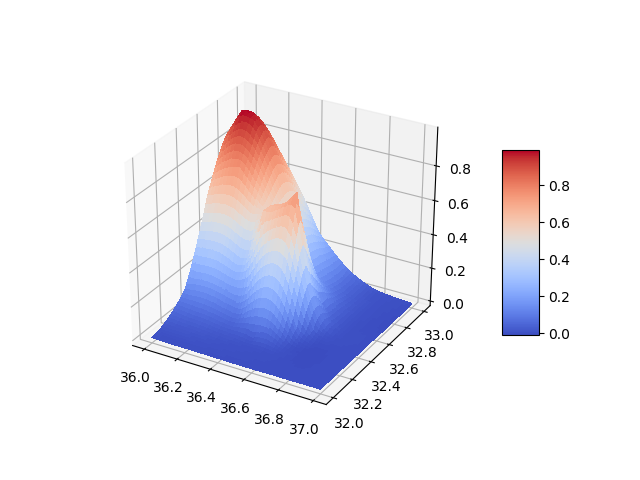
\includegraphics[width=20em]{linear_app88rbf_02.png}











Kaynaklar

[1] Neto, {\em Radial Basis Functions}, \url{http://www.di.fc.ul.pt/~jpn/r/rbf/rbf.html}

\end{document}






